\chapter{Analysis}
\label{ch:analysis}
In the analysis
phase, the product requirements are derived --- defining the client expectations
for the product --- as well as the project constraints --- what the environments
limits about the product. Finally, the theoretical foundations are outlined,
providing the basic technical knowledge to undertake the project.

% background and state of the art
%\section{Background and State of the Art}
\label{sec:background-state-art}

%\section{Theoretical foundations}
%\label{sec:theor-found}
%The theoretical foundations provide the basic technical knowledge for project
%undertaking. In that sense, it is important to understand the principle of
%operation and the related technologies, namely the infrared communication
%protocol consisting of well-established data frames, specific to each
%manufacturer and at specific bandwith. It should be highlighted that the
%communication protocol information is critical for the correct behavior of the
%TV remote control, as the latter must stimulate the TV, complying to this protocol.
%
%Pushing a button on a remote control sets in motion a series of events
%that causes the controlled device to carry out a command. The process
%can be generally described as:
%\begin{enum-c}
%\item 
%pushing the button on the remote control causes a touch to the contact beneath it and complete the button circuit on the circuit board. The integrated circuit detects this.
%\item 
%The integrated circuit sends the binary of the button function command to the
%infrared \gls{led} at the front of the remote.
%\item 
%The \gls{led} emits a series of light pulses that corresponds to the binary the button command.
%\end{enum-c}
%
%As an example, one can take a look at the clicking on the ``volume up'' button
%on a Sony TV remote (Fig.~\ref{fig:btncode}):
%%
%  %\vspace{-5mm}
%%  
%%
%\begin{figure}[htb!]
%\centering
%    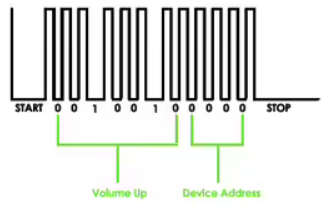
\includegraphics[width=0.45\columnwidth]{./img/buttoncode.png}
%  \caption{Example of wave generator for "volume up" from~\cite{btncode}}%
%\label{fig:btncode}
%\end{figure}
%
%The remote signal includes more than the command for ``volume up''. It sends
%several bits of information to the receiving device, establishing a
%communication protocol, including:
%\begin{item-c}
%\item a ``start'' command
%\item the command code for ``volume up''
%\item the device address (so the TV knows the data is intended for it)
%\item a ``stop'' command (triggered when you release the ``volume up'' button)
%\end{item-c}
%
%In this case, the buttons that are needed and its codes are:
%\begin{item-c}
%\item
%Power On = 001 0101
%\item
%Power Off = 010 1111
%\item
%Volume Up = 001 0010
%\item
%Volume Down = 001 0011
%\end{item-c}
%%
%  %\vspace{-5mm}
%%  
%\subsection{Reverse engineering}
%\label{sec:reverse-engineering}
%The contract established between the client (Samsung company) and the developer
%team (the authors) imposes the disclosement of the required information about
%the communication protocol. However, this is not always necessarily the case. As
%such, it is important to have a backup plan, which, in this case, corresponds to
%perform reverse engineering on the communication protocol.
%
%For this endeavour, an ``attack'' can be performed on the TV, by stimulating it
%at varying frequencies and set of commands and observing its effect. Obviously,
%the complexity grows with the number of required commands, but as in this case
%there are only 3 commands, this can be feasible. Furthermore, this can be
%bootstrapped by using available TV remote control emulators. An example setup
%can be connecting an \gls{ir} receiver at a Raspberry Pi, as illustrated in
%Fig.~\ref{fig:rasp-lirc} and loading a package, called \gls{lirc} that allows you to decode and send infrared signals of many (but not all) commonly used remote controls.
%
%The most important part of LIRC is the lircd daemon which decodes IR signals
%received by the device drivers and provides the information on a socket. It also
%accepts commands for IR signals to be sent if the hardware supports
%this~\cite{lirc}. Additionally, the sent IR signals can be used to identify the
%emitter characteristics, if already present in the database, or simply recorded
%for later usage. For the present use case, the list of available commands for
%Samsung TVs can also be obtained for the database for actual TV ``attack''.
%%
%  %\vspace{-5mm}
%%  
%%
%\begin{figure}[htb!]
%\centering
%    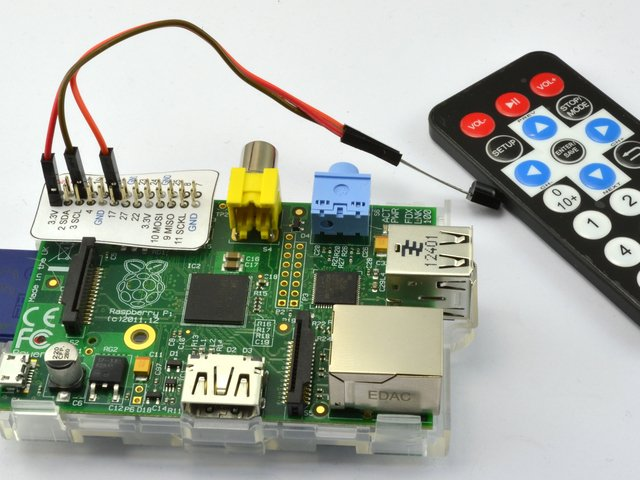
\includegraphics[width=0.43\columnwidth]{./img/rasp-reverse-engineering-setup.jpg}
%  \caption{Example setup for reverse engineering of TV remote control commands
%    using an emulator~\cite{rasp-lirc}}%
%\label{fig:rasp-lirc}
%\end{figure}

%%% Local Variables:
%%% mode: latex
%%% TeX-master: "../../../dissertation"
%%% End:

% Requirements and constraints
\section{Requirements and Constraints}
\label{sec:req-const}
%
The development requirements are divided into functional and non-functional if they pertain to main functionality or secondary one, respectively. Additionally, the constraints of the project are classified as technical or non-technical.

\subsection{Functional requirements}
\label{sec:funct-requ}
%
\begin{item-c}
\item Advertising through a screen and speakers;
\item Have fragrance diffusion;
\item Take pictures and~\gls{gif}s;
\item Detect a user in range of the device;
\item Contactless user interaction through gesture recognition;
\item Camera feed and facial recognition;
\item Apply brand-specific image filters;
\item Enable sharing multimedia across social media;
\item Provide a remote user interface for brands to purchase and configure the advertisements;
\item Provide a remote user interface for company staff to assess and control
  the MDO local system.
\end{item-c}
%
\subsection{Non-functional requirements}
\label{sec:non-funct-requ}
%
\begin{item-c}
\item Low power consumption;
\item Provide user-friendly interfaces;
\item Have low latency between local system and remote server;
\item Use wireless communication between the local and remote systems.
\end{item-c}
%
\subsection{Technical constraints}
\label{sec:techn-constr}
%
\begin{item-c}
\item Use device drivers;
\item Use Makefiles;
\item Use C/C++;
%\item Develop a~\gls{cps};
\item Use Raspberry Pi as the development board;
\item Use compatible~\gls{hw} with the development board;
\item Use buildroot;
%\item Work with Linux;
\item Social media APIs for sharing multimedia
\item Image filtering through specialized APIs.
\end{item-c}
\subsection{Non-technical constraints}
\label{sec:non-techn-constr}

\begin{item-c}
\item Project duration: one semester (circa 20 weeks); 
\item Pair work flow;
\item Limited budget;
\item Scale model prototype.
\end{item-c}

%The requirements defined the client expectations for the TV remote control,
%namely:
%\begin{item-c}
%\item Remotely operated
%\item Low weight
%\item Powered by batteries
%\item 3 buttons: Power (Off/On); Up and Down for channel selection.
%\item Infrared emitter response time (system output response time): 100 ms
%\item The TV remote may be upgraded in the future to use more buttons
%\end{item-c}
%%
%  %\vspace{-5mm}
%%  
%\section{Constraints}
%\label{sec:constraints}
%The project constraints are the limitations the environment imposes on it, namely:
%\begin{item-c}
%\item the TV remote must contain an infrared emitter (the TV already has an infrared receiver)
%\item The TV remote control must supply the required data frames imposed by the TV
%  manufacturer
%\item Data frames may not be provided by the client
%\item Security concerns are defined by the data frames and the specific
%  communication frequency imposed by the TV manufacturer
%\item 1 week deadline: 14 h
%\item Manpower: 2 people
%\item Budget:
%  \begin{itemize}
%  \item HW (parts acquisition and assembly): fixed costs --- 1 EUR/unit (1000
%    batch production)
%    \begin{itemize}
%    \item TV remote Shell
%    \item TV remote membrane
%    \item Data acquisition \& Infrared emitter PCB
%    \end{itemize}
%  \item Development: project --- 20 EUR per hour per person, totalling 560 EUR +
%    IVA
%  \end{itemize}
%\end{item-c}
%
  %\vspace{-5mm}
%  

%%% Local Variables:
%%% mode: latex
%%% TeX-master: "../../../dissertation"
%%% End:

% System overview
%%
\section{System overview}
\label{sec:system-overview}
The system overview presents a global view of the system, considering its main
features, components and interactions. It is not intended to be complete, but
rather provide a basis for the outline of the system architecture.
Fig.~\ref{fig:sys-overview} presents the \gls{mdo} system overview.
%
\begin{figure}[htb!]
\centering
    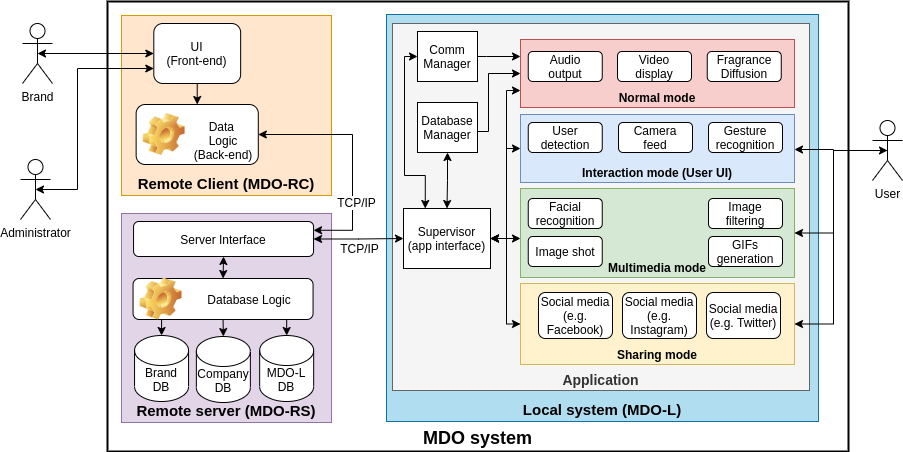
\includegraphics[width=1.0\columnwidth]{./img/sys-overview.png}
  \caption{\gls{mdo} system overview}%
\label{fig:sys-overview}
\end{figure}

Considering the system interactions, three main actors were identified:
\begin{enum-c}
\item \emph{Brand}: represents the brands contracting the advertisement
  services;
\item \emph{Administrator}: the development company staff, which can monitor and
  control the outdoor (administrative privileges).
\item \emph{User}: the user (the target audience of the advertisement)
  interacting with the system.
\end{enum-c}

Considering the data flow across the \textbf{MDO system}, three main subsystems were
identified: \textbf{\gls{mdo-rc}}, \textbf{\gls{mdo-rs}}, and
\textbf{\gls{mdo-l}}. The rational behind this initial decomposition is
explained next.

\subsection{MDO Remote Client}
The \emph{Brand} and \emph{Administrator} members require a remote \gls{ui} (front-end) to
interact with the system: the former to configure the advertisements being
displayed at the \gls{mdo} and purchase them; the latter to remotely monitor and
control the operation of the \gls{mdo}. Thus, it is clear that \emph{an
  authentication mechanism must be provided for the remote \gls{ui}}.

The data is then dispatched to the back-end, where it is processed and feed back
to the \gls{ui} user and/or sent to the remote server, via \gls{tcp-ip}
comprising the data logic component of the \gls{ui}.
%
%
\subsection{MDO Remote Server}
\label{sec:mdo-remote-server}
Although the \gls{mdo-rc} could communicate directly with the \gls{mdo-l}, this
is not desirable or a good architecture mainly due to: communications failure could
result in data loss, compromising the system's integrity; the remote client and
the local system become tightly coupled, meaning the remote client must be aware
of all the available local systems; if the data storage in the local system
fails, the remote client would have to provide the backup information.

Thus, a remote server component is included, providing the access and management
of the system databases, pertaining to the \emph{Brand}, \emph{Company}, and
\emph{MDO Local system}. The first two provide the historical information of the
\texttt{Brand} and \texttt{Administrator} entities, and the last one the information
related to all of the \texttt{\gls{mdo-l}} systems in operation.

The main functions of the \texttt{\gls{mdo-rs}} are:
\begin{item-c}
\item \emph{UI requests responses}: when a \gls{ui} user requests/modifies
  some information from the database, the server must provide/update it.
\item \emph{\gls{mdo-l} monitoring and control}: provide command dispatch and
  feedback to the \texttt{Administrator} staff for remote monitoring and control of
  the device.
\item \emph{\gls{mdo-l} update}: periodically check for start times of each
  \gls{mdo-l} device and transfer the relevant data to it.
\end{item-c}

The server interface is the responsible for managing the requests and respective
responses from the remote client and for periodically send the update data to
all \gls{mdo-l} devices. 
%
%
\subsection{MDO Local system}
\label{sec:mdo-local-system}
The \gls{mdo} local system (MDO-L) is the marketing device, interacting with the user
to display multi-sensory advertisements. As aforementioned in
Section~\ref{sec:prob-stat}, it is comprised of four modes:
\begin{item-c}
\item \emph{normal mode}: the MDO provides sound, video and fragrance
  outputs. It is the default mode.
\item \emph{interaction mode}: When a user approaches the device, the \gls{mdo} will
go into interaction mode, turning on and displaying the camera feed and waiting
for recognizable gestures to provide additional functionalities, such as
brand-specific image filters. This is the \texttt{User} \gls{ui}.
\item \emph{multimedia mode}: in this mode the facial recognition is applied,
  enabling the user to select and apply different brand-specific image filters and take pictures or create a \gls{gif}.
\item \emph{sharing mode}: after a user take a picture or create a \gls{gif}, it
  can share it across social media.
\end{item-c}

The user interaction is considered to be a higher priority activity than the
advertisements, so when a \texttt{User} interacts with the system, the \texttt{normal
mode} is overriden by the \texttt{Interaction mode}, thus, halting the
advertisements.

The \gls{mdo-l} application communicates with the remote server
(\texttt{\gls{mdo-rs}}) through the \texttt{Supervisor} via \gls{tcp-ip}
 to handle requests from \texttt{Administrator} members
to monitor and control the device through the \texttt{Supervisor} or to update
the advertisements. Additionally, the \texttt{Supervisor} oversees the
application mode and the communication (\texttt{Comm Manager}) and database
(\texttt{Database manager}) managers to handle system events.
%
%%% Local Variables:
%%% mode: latex
%%% TeX-master: "../../../dissertation"
%%% End:

% System Architecture
%%
\section{System architecture}
\label{sec:system-architecture}
In this section, the system architecture is devised in the \gls{hw} and \gls{sw} components, using the system overview as a starting point. 

\subsection{Hardware architecture}
\label{sec:hardw-arch}
%
The diagram in Fig.\ref{fig:hw-arch} represents an initial hardware big picture in order to facilitate the objective identification.
As it can bee seen, the diagram is divided in four distinguished parts: \emph{External Environment}, \emph{Local System}, \emph{Remote Server} and \emph{Remote Client}.

Firstly, the \texttt{External Environment} represents all the environment that interacts with the system. In this case, these are all its users - normal users, brands and staff.

Secondly, the \texttt{Local System} is composed for the main controller, which is the Raspberry Pi 4B. 
This \gls{mcu} is responsible to controll all the Local System and to establish connection with the remote server through its included WiFi module. 
The board is powered connecting it to the electrical network. 
Then, it has several blocks connected to it:
%
\begin{item-c}
\item \emph{Motion Detection}: Used to detect the users and switch from normal mode to interaction mode;
\item \emph{Fragrance Diffusion Actuator}: used to diffuse the fragrance onto the air;
\item \emph{Camera}: Used to capture image that is then processed;
\item \emph{Speakers}: Used to produce advertisements sounds;
\item \emph{Screen}: Used to produce video clips of advertisements.
\end{item-c}
%

In third place, the \texttt{Remote Server} has a server node running in another machine that can be one computer or a main frame.
The remote server establishes connection with the cloud that has stored all the data from all databases.

Lastly, the \texttt{Remote Client} which can be a computer, a tablet or a smart phone to run the \gls{mdo} management application.
%
\begin{figure}
\centering
    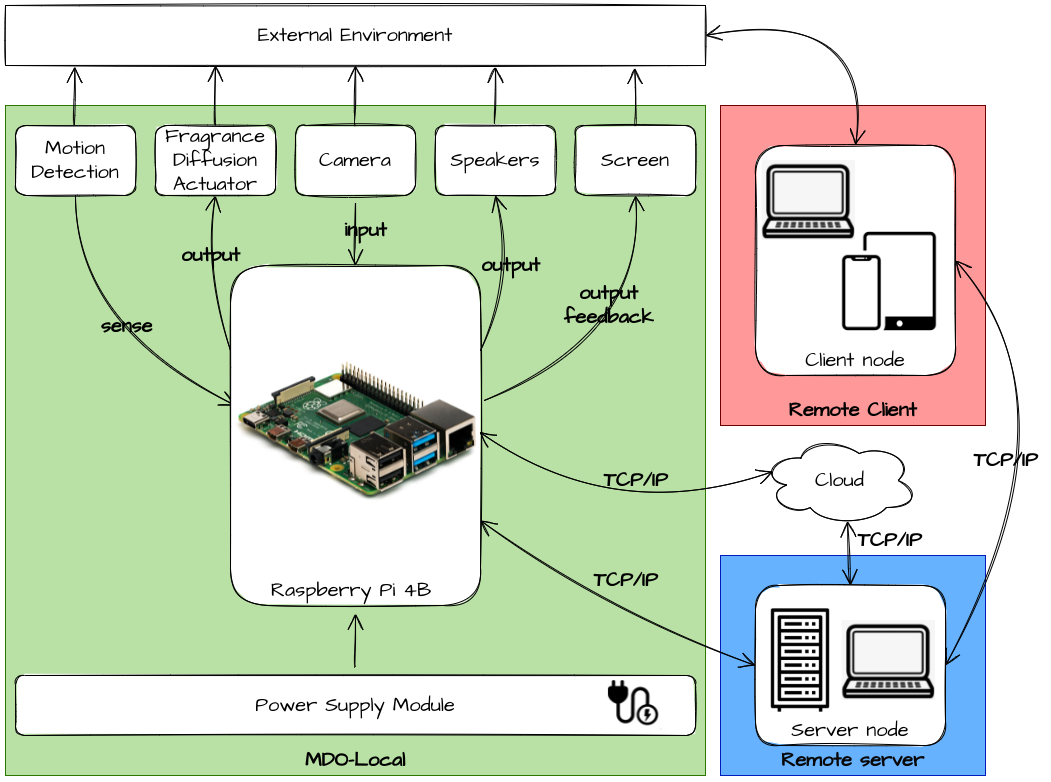
\includegraphics[width=0.9\columnwidth]{./img/HW_Architecture.png}
  \caption{~\gls{hw} Architecture Diagram}%
\label{fig:hw-arch}
\end{figure}
%
%
\subsection{Software architecture}
\label{sec:softw-arch}
In this section the \gls{sw} architecture for \gls{mdo-rc}, \gls{mdo-rs}, and
\gls{mdo-l} subsystems is presented, defining its \gls{sw} stack.

\subsubsection{MDO remote client}
\label{sec:mdo-remote-client}
Fig.~\ref{fig:sw-arch-rc} illustrates the \gls{sw} architecture for the remote
client, representing its \gls{sw} stack.
It is comprised of the following layers:
\begin{item-c}
\item \emph{Application}: contains the remote client application. The
  \texttt{Brand} and \texttt{Admin} members interact with the \gls{ui}, which is
  the visual part of the interface. The \texttt{\gls{ui} engine} is notified and
  handles all \gls{ui} events --- internal or external --- providing the \texttt{UI}
  with feedback for its users. The relevant commands
  are then parsed --- \texttt{Parser} component --- and responded. The commands
  are then translated to the appropriate \gls{db} queries and responded through
  the \texttt{DB Manager}. The \texttt{Comm Manager} is responsible for
  encapsulating the \gls{db} queries into the respective \gls{tcp-ip} frames to
  be sent to the \texttt{Remote Server} as well as unwrap the incoming server
  responses.
\item \emph{Middleware}: contains the \gls{tcp-ip} framework supporting these
  communication protocols as part of \gls{osi} model for internet
  applications. It manages the incoming/outgoing \gls{tcp-ip} frames by
  providing the adequate protocol handshaking and queueing and timing aspects of
  the bytes to send/receive.
\item \emph{OS \& BSP} --- \gls{os} \& \gls{bsp}: it contains the low-level and
  communication drivers required to handle input (keyboard/touch), output
  (screen) and communication to the \texttt{Remote Server}.
\end{item-c}
It should be noted that for desktop and mobile applications, the
\texttt{Middleware} and \texttt{OS \& BSP} layers are usually abstracted by the
\gls{os}, thus, the relevant \gls{api}s should be used.
%
\begin{figure}
\centering
    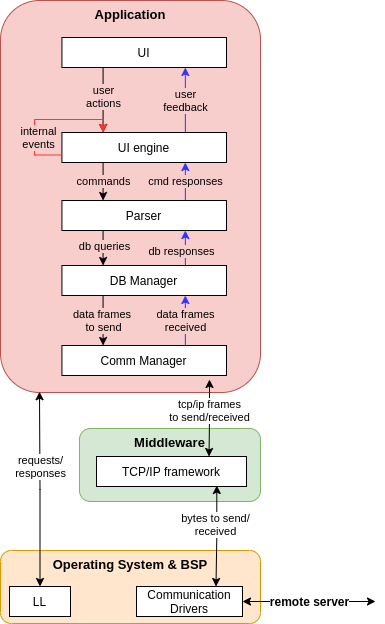
\includegraphics[width=0.55\columnwidth]{./img/sw-arch-rc.png}
  \caption{~\gls{sw} architecture diagram: remote client}%
\label{fig:sw-arch-rc}
\end{figure}

\subsubsection{MDO remote server}
\label{sec:mdo-remote-server-1}
%
Fig.~\ref{fig:sw-arch-rs} illustrates the \gls{sw} stack for architecture for
the remote server.
It is comprised of the following layers:
\begin{item-c}
\item \emph{Application}: contains the remote server application. It provides a
  \gls{cli} to handle \texttt{Remote client} requests.  The \gls{cli} engine
  is notified and handles all \gls{ui} events --- internal or external ---
  providing the appropriate feedback. The relevant commands
  are then parsed --- \texttt{Parser} component --- and responded: \gls{db}
  queries are handled by the \texttt{\gls{rdbms}} issuing \gls{db} transactions;
  other commands received by the \texttt{Remote Client} are handled internally
  and translated, being dispatched to the \texttt{Local
    System} by the \texttt{Comm Manager}  (via \texttt{Communication drivers}). Internal events can also
  trigger the \texttt{\gls{rdbms}} to issue database transactions for the
  \texttt{Remote Client} or \texttt{Local System}.
  The \texttt{Comm Manager} is responsible for wrapping\slash unwrapping the data
  frames received by or sent to the \texttt{Remote Client} or \texttt{Local System}.
\item \emph{Middleware}: contains the \gls{rdbms} framework supporting the
  management of the relational databases using database transactions.
\item \emph{OS \& BSP} --- \gls{os} \& \gls{bsp}: it contains the \texttt{Communication}
  drivers to the handle requests from the \texttt{Remote Client}, and the
  \texttt{File I/O} drivers to manipulate \gls{db} transactions from\slash to storage.
\end{item-c}
%
\begin{figure}
\centering
    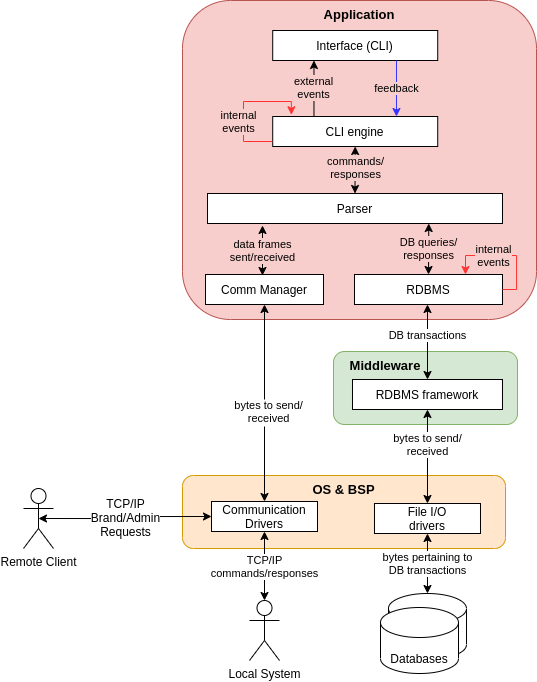
\includegraphics[width=0.55\columnwidth]{./img/sw-arch-rs.png}
  \caption{~\gls{sw} architecture diagram: remote server}%
\label{fig:sw-arch-rs}
\end{figure}
%
\subsubsection{MDO local system}
\label{sec:mdo-local-system-1}




%%% Local Variables:
%%% mode: latex
%%% TeX-master: "../../../dissertation"
%%% End:

% Subsystem decomposition
%
\section{Subsystem decomposition}
\label{sec:subsyst-decomp}

For each subsystem, do:
1. Events
2. Use cases
3. State machine diagram
4. Sequence diagram

\subsection{Local system}
\label{sec:local-system}

\subsubsection{Events}
\label{sec:events}

\subsubsection{Use cases}
\label{sec:use-cases}

\subsubsection{Dynamic operation}
\label{sec:dyn-oper}
State machine diagram

\subsubsection{Flow of events}
\label{sec:flow-events}
Sequence diagram

\subsection{Remote system}
\label{sec:remote-system}

\subsubsection{Events}
\label{sec:events-1}

\subsubsection{Use cases}
\label{sec:use-cases-1}

\subsubsection{Dynamic operation}
\label{sec:dyn-oper-1}
State machine diagram

\subsubsection{Flow of events}
\label{sec:flow-events-1}
Sequence diagram


%%% Local Variables:
%%% mode: latex
%%% TeX-master: "../../../dissertation"
%%% End:

% Project planning and budget
%\section{Project planning}
\label{sec:project-planning}

\subsection{Budget}
\label{sec:budget}


%%% Local Variables:
%%% mode: latex
%%% TeX-master: "../../../dissertation"
%%% End:

%%% Local Variables:
%%% mode: latex
%%% TeX-master: "../../../dissertation"
%%% End:
